%%%%%%%%%%%%%%%%%%%%%%%%%%%%%%%%%%%%%%%%%
% Beamer Presentation
% LaTeX Template
% Version 1.0 (10/11/12)
%
% This template has been downloaded from:
% http://www.LaTeXTemplates.com
%
% License:
% CC BY-NC-SA 3.0 (http://creativecommons.org/licenses/by-nc-sa/3.0/)
%
%%%%%%%%%%%%%%%%%%%%%%%%%%%%%%%%%%%%%%%%%

%----------------------------------------------------------------------------------------
%	PACKAGES AND THEMES
%----------------------------------------------------------------------------------------

\documentclass{beamer}

\mode<presentation> {

% The Beamer class comes with a number of default slide themes
% which change the colors and layouts of slides. Below this is a list
% of all the themes, uncomment each in turn to see what they look like.

%\usetheme{default}
%\usetheme{AnnArbor}
%\usetheme{Antibes}
%\usetheme{Bergen}
%\usetheme{Berkeley}
%\usetheme{Berlin}
%\usetheme{Boadilla}
%\usetheme{CambridgeUS}
%\usetheme{Copenhagen}
%\usetheme{Darmstadt}
%\usetheme{Dresden}
%\usetheme{Frankfurt}
%\usetheme{Goettingen}
%\usetheme{Hannover}
%\usetheme{Ilmenau}
%\usetheme{JuanLesPins}
%\usetheme{Luebeck}
\usetheme{Madrid}
%\usetheme{Malmoe}
%\usetheme{Marburg}
%\usetheme{Montpellier}
%\usetheme{PaloAlto}
%\usetheme{Pittsburgh}
%\usetheme{Rochester}
%\usetheme{Singapore}
%\usetheme{Szeged}
%\usetheme{Warsaw}

% As well as themes, the Beamer class has a number of color themes
% for any slide theme. Uncomment each of these in turn to see how it
% changes the colors of your current slide theme.

%\usecolortheme{albatross}
%\usecolortheme{beaver}
%\usecolortheme{beetle}
%\usecolortheme{crane}
%\usecolortheme{dolphin}
%\usecolortheme{dove}
%\usecolortheme{fly}
%\usecolortheme{lily}
%\usecolortheme{orchid}
%\usecolortheme{rose}
%\usecolortheme{seagull}
%\usecolortheme{seahorse}
%\usecolortheme{whale}
%\usecolortheme{wolverine}

%\setbeamertemplate{footline} % To remove the footer line in all slides uncomment this line
%\setbeamertemplate{footline}[page number] % To replace the footer line in all slides with a simple slide count uncomment this line

%\setbeamertemplate{navigation symbols}{} % To remove the navigation symbols from the bottom of all slides uncomment this line
}

\usepackage{graphicx} % Allows including images
\usepackage{booktabs} % Allows the use of \toprule, \midrule and \bottomrule in tables
\usepackage{color, colortbl}
\usepackage{graphicx}
%----------------------------------------------------------------------------------------



%	TITLE PAGE
%----------------------------------------------------------------------------------------

%\title[Six Algorithms]{Six Algorithms \\ \footnotesize Select Typical Machine Learning Algorithms for Data Analytics} % The short title appears at the bottom of every slide, the full title is only on the title page

\title[PaperReading:MIC-SVM]{PaperReading}
\subtitle{MIC-SVM:Designing a highly efficient support vector machine for advanced modern multi-core and many-core architectures \\
Y. You et al., IPDPS 2014}

\author{Bo Peng} % Your name
\institute[IUB] % Your institution as it will appear on the bottom of every slide, may be shorthand to save space
{
Digital Science Center \\
Indiana University\\ % Your institution for the title page
\medskip
\textit{pengb@indiana.edu} % Your email address
}
\date{\today} % Date, can be changed to a custom date

\begin{document}
	

%----------------------------------------------------------------------------------------
%	PRESENTATION SLIDES
%----------------------------------------------------------------------------------------
\begin{frame}
	\maketitle
\end{frame}

\AtBeginSubsection[]
{
	\begin{frame}
		\frametitle{Outline} % Table of contents slide, comment this block out to remove it
		\tableofcontents[currentsection,currentsubsection, 
		sectionstyle=show/shaded,
		] % Throughout your presentation, if you choose to use \section{} and \subsection{} commands, these will automatically be printed on this slide as an overview of your presentation
	\end{frame}
} 
%------------------------------------------------
\section{Background of the paper} % Sections 
\subsection{the Authors} 
\begin{frame}
	\frametitle{the Authors}
	\begin{columns}[c] % The "c" option specifies centered vertical alignment while the "t" option is used for top vertical alignment
		
		\column{.45\textwidth} % Left column and width
		%\textbf{Heading}
		\begin{figure}
			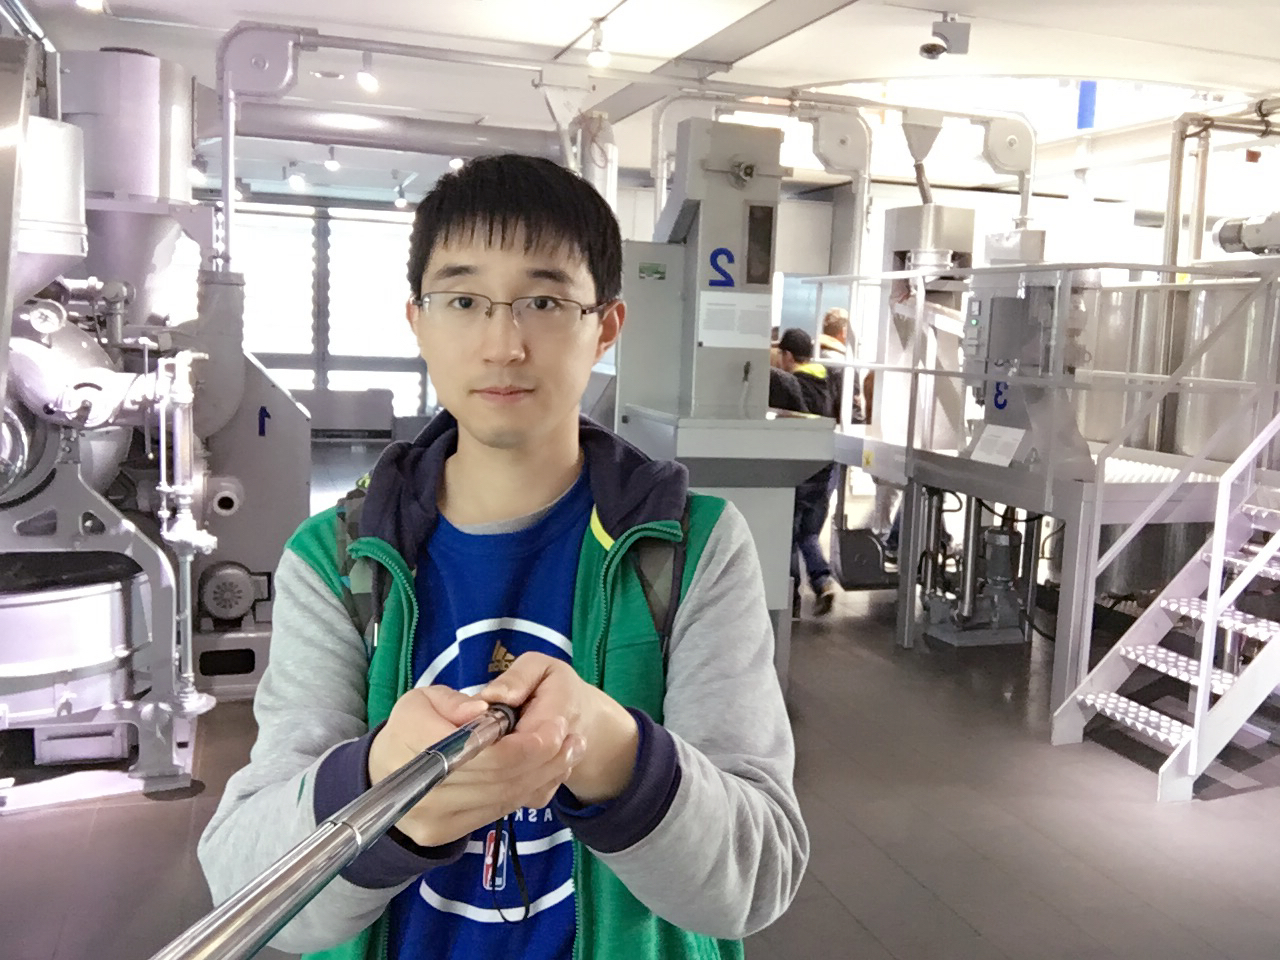
\includegraphics[width=1\linewidth]{figs/yangyou2.jpg}
			%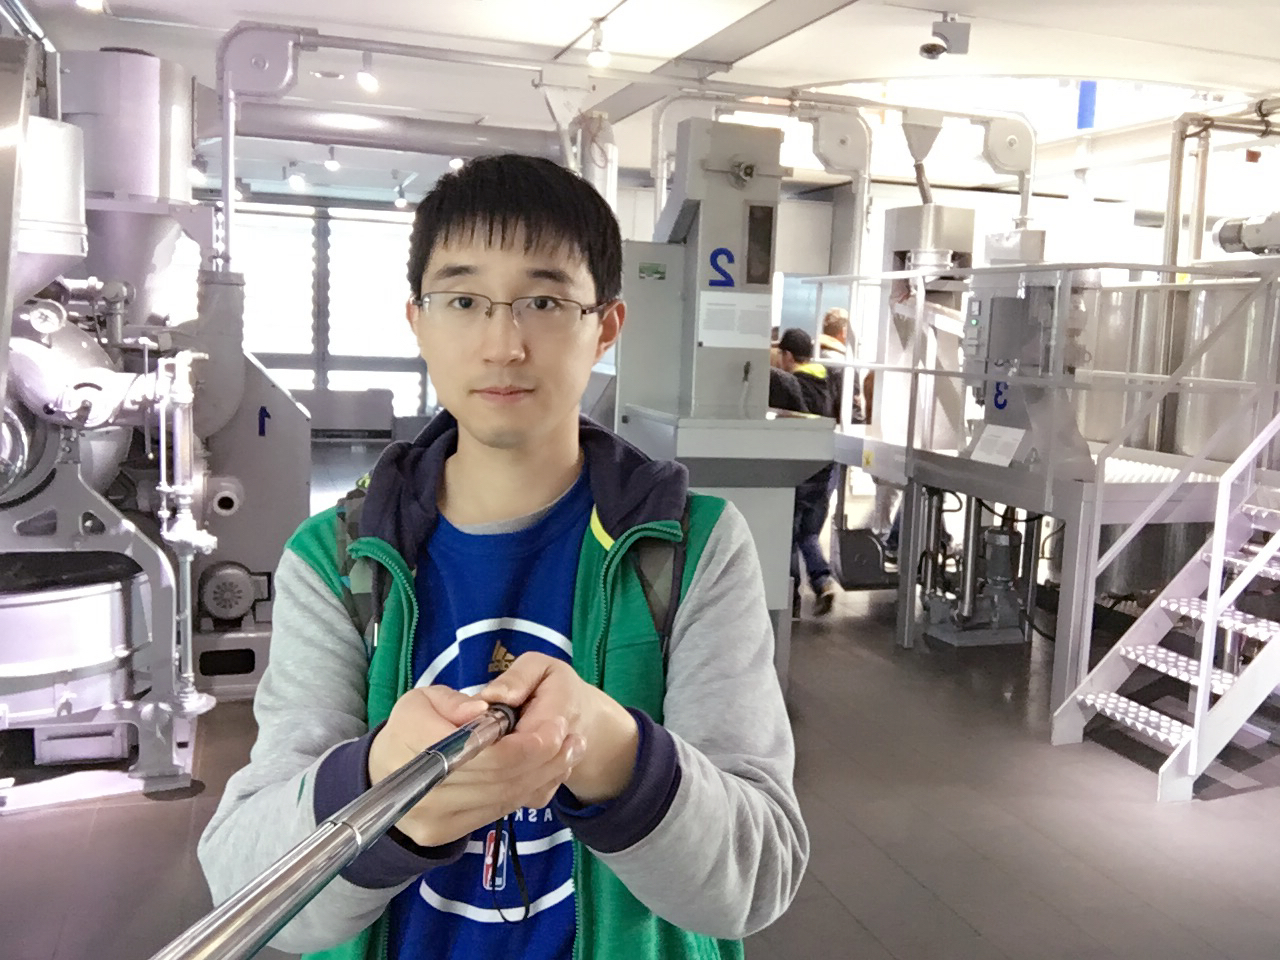
\includegraphics[width=3.4cm,height=3.4cm]{figs/yangyou2.jpg}		
		\end{figure}
		
		\column{.5\textwidth} % Right column and width
		\begin{itemize}
			\item \href{https://people.eecs.berkeley.edu/~youyang/}{\textcolor{blue}{Yang You}}, PhD student at UC Berkeley CS, Master 2015 Tsinghua
			\item research interests include Parallel Computing, Distributed Systems, and Machine Learning
			\item  CA-SVM: Communication-Avoiding Support Vector Machines on Distributed Systems.  \textcolor{red}{Best Paper IPDPS 2015}  
			
		\end{itemize}
		
	\end{columns}	
\end{frame}

\begin{frame}
	\frametitle{the Authors}
	\begin{columns}[c] % The "c" option specifies centered vertical alignment while the "t" option is used for top vertical alignment
		
		\column{.45\textwidth} % Left column and width
		%\textbf{Heading}
		\begin{figure}
			%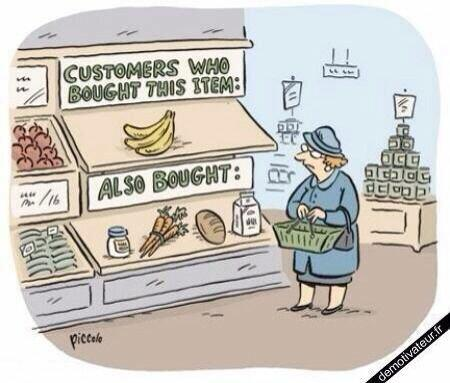
\includegraphics[width=0.7\linewidth]{fig/Humor_recommender.jpg}
			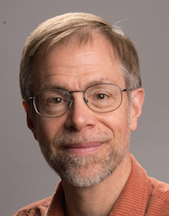
\includegraphics[width=0.7\linewidth]{figs/Demmel_2015_photo_v5.png}
		\end{figure}
		
		\column{.5\textwidth} % Right column and width
		\begin{itemize}
			\item \href{https://people.eecs.berkeley.edu/~demmel/}{\textcolor{blue}{Prof. James Demmel}} \\Computer Science Division Chair, and EECS Associate Chair,Professor of Mathematics and Computer Science 
			\item Research Projects:
			Communication-Avoiding Algorithms \\
			The Complexity of Accurate Floating Point Computation \\
			%http://www.netlib.org/lapack/contributor-list.html
			%Jim Demmel (University of California, Berkeley; US),
			%Inderjit Dhillon (University of California, Berkeley; US),
			LAPACK, scaLAPACK, main contributor
		\end{itemize}
		
	\end{columns}	
\end{frame}

\begin{frame}
	\frametitle{the Authors: BeBOP Group}
	\href{http://bebop.cs.berkeley.edu/}{\textcolor{blue}{BeBOP}}(Berkeley Benchmarking and OPtimization Group) \\
	The BeBOP group is broadly interested in understanding software performance tuning issues, and the interaction or implications for hardware design. Among our general interests are
		\begin{itemize}
			\item 	
	the interaction between application software, compilers, and hardware
	managing trade-offs among the various measures of performance, such as speed, accuracy, power, storage, ...
				\item 
	automating the performance tuning process, starting with the computational kernels which dominate application performance in scientific computing and information retrieval
				\item 
	performance modeling and evaluation of future computer architectures
			\end{itemize}
\end{frame}


\section{Work of the paper} % Sections 
\subsection{I. Introduction} 
\begin{frame}
	\frametitle{Motivations}
	Mic-svm: Designing a highly efficient support vector machine for advanced modern multi-core and many-core architectures
	\begin{block}{Motivation}
		\begin{itemize}
			\item svm is important...widely used...recently being used in HPC for performance and power...
			prediction
			\item challenge
			of scaling performance over tens or even hundreds of cores within a
			single chip
			\item there has been
			no efficient SVM tool designed for advanced x86 based multi- and
			many-core architectures
		\end{itemize}		
	\end{block}
	
\end{frame}


\begin{frame}
	\frametitle{Research Problem}
	\begin{block}{Problems to solve(...unwritten...)}
		\begin{itemize}
			\item What's the problem? --svm train phase inefficient in x-core system
			\item What's the state-of-art solutions? -- libsvm, gpusvm
			\item What's the deficiency of those solutions? -- 
			\item What's the \textcolor{red}{methodology} to investigate these performance issues? -- bottleneck, profiling, bound analysis, ...
			\item What's the suitable \textcolor{red}{optimization techniques}?
			\item What's a good \textcolor{red}{mapping} from input data pattern to specific architecture and optimization decisions?
		\end{itemize}		
	\end{block}
	
\end{frame}

\begin{frame}
	\frametitle{Contributions}
	\begin{block}{Contributions}
		\begin{itemize}
			\item Designing and implementing MIC-SVM a highly efficient parallel...
			\item Proposing \textcolor{red}{novel analysis methods} and \textcolor{red}{optimization techniques}
			(i.e. adaptive support for input patterns and data parallelism) to
			fully utilize the multi-level parallelism provided by the studied
			architectures.
			\item Exploring and improving the deficiencies of the current tool...
			\item Providing insights on \textcolor{red}{how to select the most suitable architectures} for specific algorithms and input data patterns to achieve
			best performance.
		\end{itemize}		
	\end{block}
	
\end{frame}

\subsection{II. Background of SVM} % Sections can be created in order to organize your presentation into discrete blocks, all sections and subsections are automatically printed in the table of contents as an overview of the talk

\begin{frame}
	\frametitle{Classification Problems}
	\begin{columns}[c] % The "c" option specifies centered vertical alignment while the "t" option is used for top vertical alignment
		
		\column{.4\textwidth} % Left column and width
		%\textbf{Heading}
		\begin{figure}
			%\includegraphics[width=0.6\textwidth]{fig/"l1l2".jpg}
			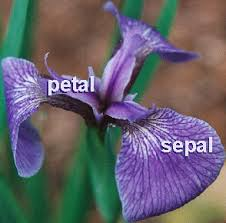
\includegraphics[width=1\textwidth]{figs/iris-petal.jpg}
			
			%\footnotesize {Logistic Regression}				
		\end{figure}
		
		\column{.6\textwidth} % Right column and width
		IRIS Dataset
		\begin{figure}
			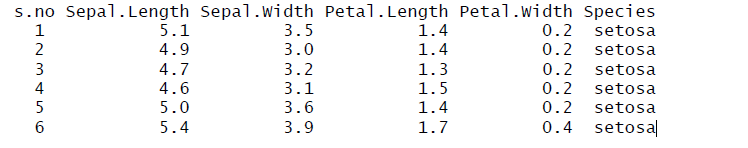
\includegraphics[width=1.0\textwidth]{figs/irisdata.png} \\
			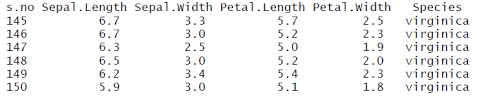
\includegraphics[width=1.0\textwidth]{figs/irisdata2.png}
		\end{figure}			
	\end{columns}	
	
	\begin{itemize}
		\item features: \{sepal.length, sepal.width, petal.length, petal.width\}. 
		\item lables: \{setosa, virginica\}
		\item task: predict label by observed data with the fetures
	\end{itemize}	
	
	
\end{frame}


\begin{frame}
	\frametitle{SVM(Support Vector Machine)}
	\begin{columns}[c] % The "c" option specifies centered vertical alignment while the "t" option is used for top vertical alignment
	
	\column{.6\textwidth} % Left column and width
	%\textbf{Heading}
	\begin{figure}
		%\includegraphics[width=0.6\textwidth]{fig/"l1l2".jpg}
		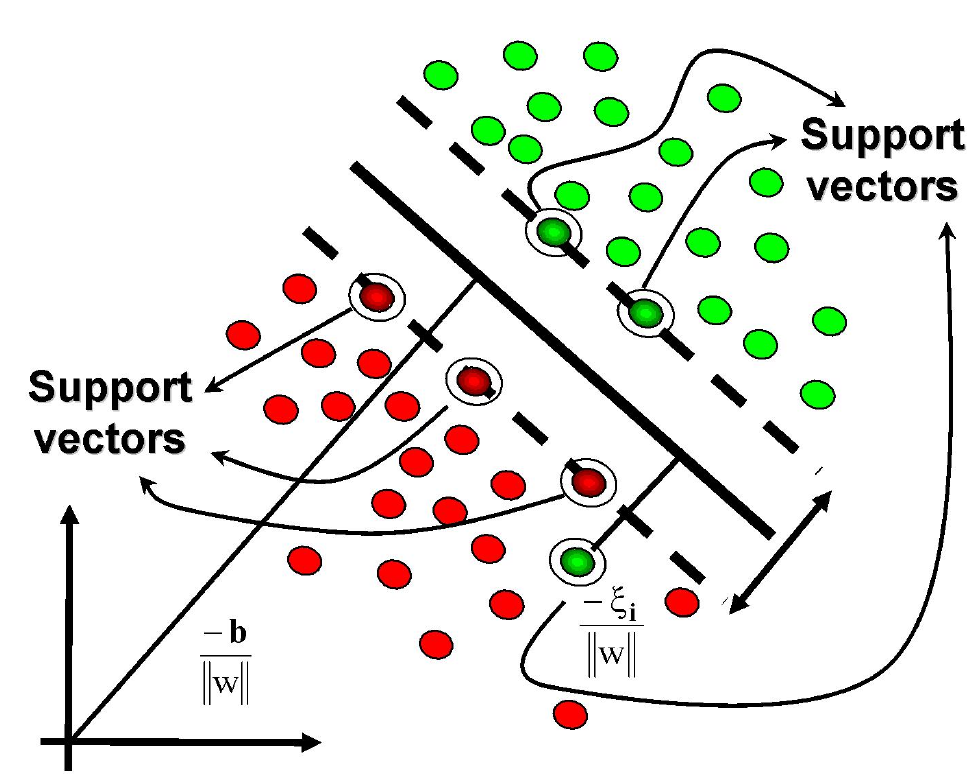
\includegraphics[width=0.8\textwidth]{figs/fig1_svm.png}
		
		%\footnotesize {Logistic Regression}				
	\end{figure}
	
	\column{.4\textwidth} % Right column and width
		\begin{itemize}
		\item separation plane: $y = \vec{w} \cdot \vec{x} - b$
		\item separation with maximum margin
		\item finally, we will get: \\
		%normal vector \vec{w}
		$\vec w = \sum_{i=1}^n \alpha_iy_i \vec x_i$	\\
		$\vec w$ can be written as a linear combination of the \textcolor{red}{support vectors}.
		\end{itemize}			
	\end{columns}	
	
	\begin{itemize}
		\item a representation of the examples as points in space, mapped so that the examples of the separate categories are divided by a clear gap that is \textcolor{red}{as wide as possible}. 
		\item $\arg\min_{\vec{w},b} \left\{\frac 1 2 \lVert \vec{w} \rVert^2 \right\} \text{subject to } y_i(\vec{w}\cdot\vec{x_i}-b) \geq 1, \forall i$	
		%with slack variable
		\item $\arg\min_{\vec{w},b,\xi} \left\{\frac 1 2 \lVert \vec{w} \rVert^2 + C\sum_{i=1}^{n}\xi_i \right\} \text{subject to } y_i(\vec{w}\cdot\vec{x_i}-b) \geq 1-\xi_i, \forall i$	
			
		%lagrange multipliers
		%\item $\arg\min_{\vec{w}} \left\{ \frac 1 n \sum_{i=1}^n \max\left(0, 1 - y_i(\vec{w}\cdot \vec{x_i} + b)\right) + \lambda\lVert \vec{w} \rVert^2 \right\}$		
	\end{itemize}	
	
	
\end{frame}



\begin{frame}
	\frametitle{SVM: Kernel Trick}
	\begin{columns}[c] % The "c" option specifies centered vertical alignment while the "t" option is used for top vertical alignment
	
	\column{.6\textwidth} % Left column and width
	%\textbf{Heading}
	\begin{figure}
		%\includegraphics[width=0.6\textwidth]{fig/"l1l2".jpg}
		\includegraphics[width=0.9\textwidth]{fig/"svm_kerneltrick03".png}
		
		%\footnotesize {Logistic Regression}				
	\end{figure}
	
	\column{.4\textwidth} % Right column and width
	%\begin{itemize}
	$k(\mathbf{x}, \mathbf{x'})$ \\
    $= \langle \mathbf{x},\mathbf{x'} \rangle^2 $ \\
	$= (\mathnormal{x}_1\mathnormal{x'}_1 + \mathnormal{x}_2\mathnormal{x'}_2)^2 $ \\
	$= \mathnormal{x}_1^2\mathnormal{x'}_1^2+ \sqrt{2}{\mathnormal{x}_1\mathnormal{x}_2}\sqrt{2}{\mathnormal{x'}_1\mathnormal{x'}_2} $ \\
	$   + \mathnormal{x}_2^2\mathnormal{x'}_2^2 $ \\
	$= \langle \varphi(\mathbf{x}), \varphi(\mathbf{x'}) \rangle$
    
		%$k(\mathbf{x}, \mathbf{x'}) \\
		    %= \langle \mathbf{x},\mathbf{x'} \rangle^2 \\
		    %= (x_1x'_1 + x_2x'_2)^2  \\
		    %= x_{1}^2x'_{1}^2+ \sqrt{2}{x_1x_2}\sqrt{2}{x'_1x'_2}    + x_{2}^2x'_{2}^2  \\
			%= \langle \varphi(\mathbf{x}), \varphi(\mathbf{x'}) \rangle$
			
			
	%\end{itemize}			
	\end{columns}	
	
	\begin{itemize}
		\item $\hat{y} = \vec{w}\cdot\vec{x}-b = \sum_{i=1}^n \alpha_i y_i k(\mathbf{x}_i, \mathbf{x'})-b$, for $k(\mathbf{x}, \mathbf{x'}) = \langle \varphi(\mathbf{x}), \varphi(\mathbf{x'}) \rangle_\mathcal{V}$
		\item use of kernel functions, which enable them to operate in a high-dimensional, implicit feature space without ever computing the coordinates of the data in that space, but rather by simply computing the \textcolor{red}{inner products} between the images of all pairs of data in the feature space. 
	\end{itemize}	
	
\end{frame}

\begin{frame}
	\frametitle{Numerical Optimization Problem}
	......transformed into the dual form
	
	\begin{itemize}
		\item QP(Quadratic programming) problem
		\item training phase \\
		%Quadratic programming (QP) is the process of solving a special type of mathematical optimization problem—specifically, a (linearly constrained) quadratic optimization problem, that is, the problem of optimizing (minimizing or maximizing) a quadratic function of several variables subject to linear constraints on these variables. Quadratic programming is a particular type of nonlinear programming.
		$\text{Maximize: } F(\alpha)=\sum_{i=1}^{n}\alpha_i- \frac 1 2 \sum_{i=1}^{n}\sum_{j=1}^{n}\alpha_i\alpha_jy_iy_jKernel(X_i,X_j)$ \\ $\text{subject to: } \sum_{i=1}^{n}\alpha_iy_i=0 \text{ and } 0 \leq \alpha_i \leq C, \forall i$	
		\item prediction phase \\
			$ \text{predict: } \hat{y_i} = u_i = \sum_{j=1}^{n}\alpha_jy_jK(\vec{x_j},\vec{x_i})-b $
	
	\end{itemize}	
	
\end{frame}

\begin{frame}
	\frametitle{SMO(Sequential Minimal Optimization) Algorithm}	 
	\begin{itemize}
		\item At every step, SMO chooses \textcolor{red}{two} Lagrange multipliers to jointly optimize, finds the
		optimal values for these multipliers, and updates the SVM to reflect the new optimal values
		
		\begin{columns}[c] % The "c" option specifies centered vertical alignment while the "t" option is used for top vertical alignment
			
			\column{.2\textwidth} % Left column and width
				\text{subject to: } \\
				$\sum_{i=1}^{n}\alpha_iy_i=0$ \\
				\text{ and } \\
				$0 \leq \alpha_i \leq C, \forall i$	
			
			\column{.8\textwidth} % Right column and width
				\begin{figure}
					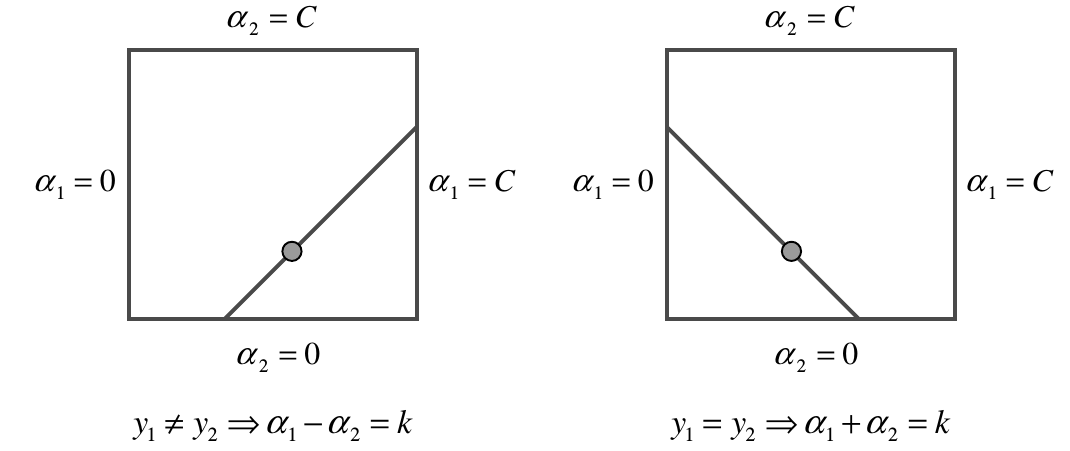
\includegraphics[width=0.8\textwidth]{figs/two_lagrange_opt.png}
					%\footnotesize {Logistic Regression}				
				\end{figure}
		\end{columns}
		\item 
		The inequality constraints cause the Lagrange multipliers to lie in the box. The linear equality
		constraint causes them to lie on a diagonal line. Therefore, one step of SMO must find an
		optimum of the objective function on \textcolor{red}{a diagonal line segment}.
	\end{itemize}	
\end{frame}

\begin{frame}
	\frametitle{SMO: Update Equation}	 
	\begin{itemize}
		\item The second derivative of the objective function along the diagonal line can be expressed as:
		$\eta = K(\vec{x_1},\vec{x_1})+K(\vec{x_2},\vec{x_2})-2K(\vec{x_1},\vec{x_2})$ 
		\item $\alpha_{2}^{new} = \alpha_2 + \frac{y_2(E_1-E_2)}{\eta}$ \text{ where } $E_i = u_i-y_i $ is the error on ith training example 
		\item $\alpha_{1}^{new} = \alpha_1 + y_1y_2(\alpha_2-\alpha_{2}^{new})$

		\item $E_{i}^{new} = E_i + (\alpha_{1}^{new}-\alpha_1)y_1K(\vec{X_1},\vec{X_i}) + (\alpha_{2}^{new}-\alpha_2)y_2K(\vec{X_2},\vec{X_i})$	
		\item more deatils refer to \cite{Platt}
		
	\end{itemize}	
	
	
\end{frame}



\begin{frame}
	\frametitle{SMO:selection of the two lagrange multipliers}	 

		\begin{columns}[c] % The "c" option specifies centered vertical alignment while the "t" option is used for top vertical alignment
			
			\column{.5\textwidth} % Left column and width
			%\textbf{Heading}
			\begin{figure}
				%\includegraphics[width=0.6\textwidth]{fig/"l1l2".jpg}
				\includegraphics[width=0.9\textwidth]{figs/"fig1_svm".png}
				
				%\footnotesize {Logistic Regression}				
			\end{figure}
			
			\column{.5\textwidth} % Right column and width
			
			The Karush-Kuhn-Tucker (KKT) conditions are \textcolor{red}{necessary and sufficient conditions} for an
			optimal point of a positive definite QP problem. \\
			$ \text{set: } u_i = \sum_{j=1}^{n}\alpha_jy_jK(\vec{x_j},\vec{x_i})-b, $\\ \text{ then}
			
			$ \alpha_i=0 \Leftrightarrow y_iu_i \geq 1, $ \\
			$ 0 < \alpha_i < C \Leftrightarrow y_iu_i = 1,$\\
			$ \alpha_i=C \Leftrightarrow y_iu_i \leq 1,$
		\end{columns}
			\begin{itemize}
		\item chooses the first one by iterating over the entire training set, determining whether each example \textcolor{red}{violates the KKT
		conditions}.
		\item chooses the second one with \textcolor{red}{maximized step size} which is approximated by the absolute value of error $|E_1-E_2|$.
	\end{itemize}	
\end{frame}

\begin{frame}
	\frametitle{SMO:selection equations}	 

	\begin{itemize}
		\item (KKT) conditions \\
				$ \text{set: } u_i = \sum_{j=1}^{n}\alpha_jy_jK(\vec{x_j},\vec{x_i})-b,$ \\
				$ \alpha_i=0 \Leftrightarrow y_iu_i \geq 1, $ \\
				$ 0 < \alpha_i < C \Leftrightarrow y_iu_i = 1,$ \\
				$ \alpha_i=C \Leftrightarrow y_iu_i \leq 1,$
		\item group the examples into two sets: \\
				$I_1=\{i:0<\alpha_i<C\}\cup\{i:y_i>0,\alpha_i=0\}\cup\{i:y_i<0,\alpha_i=C\}$ \\
				where $E_i=u_i-y_i \geq 0$ otherwise voilate KKT cond.  \\
				
				$I_2=\{i:0<\alpha_i<C\}\cup\{i:y_i<0,\alpha_i=0\}\cup\{i:y_i>0,\alpha_i=C\}$ \\	
				where $E_i=u_i-y_i \leq 0$ otherwise voilate KKT cond.
				
		\item selection equations: \\
			$i_1 =\arg\min_{i}\{E_i:i \in I_1\}$ \\
			$i_2 =\arg\max_{i}\{E_i:i \in I_2\}$
	\end{itemize}	
\end{frame}

\begin{frame}
	\frametitle{SMO:Algorithm PseudoCode}	
	\begin{figure}
		%\includegraphics[width=0.6\textwidth]{fig/"l1l2".jpg}
		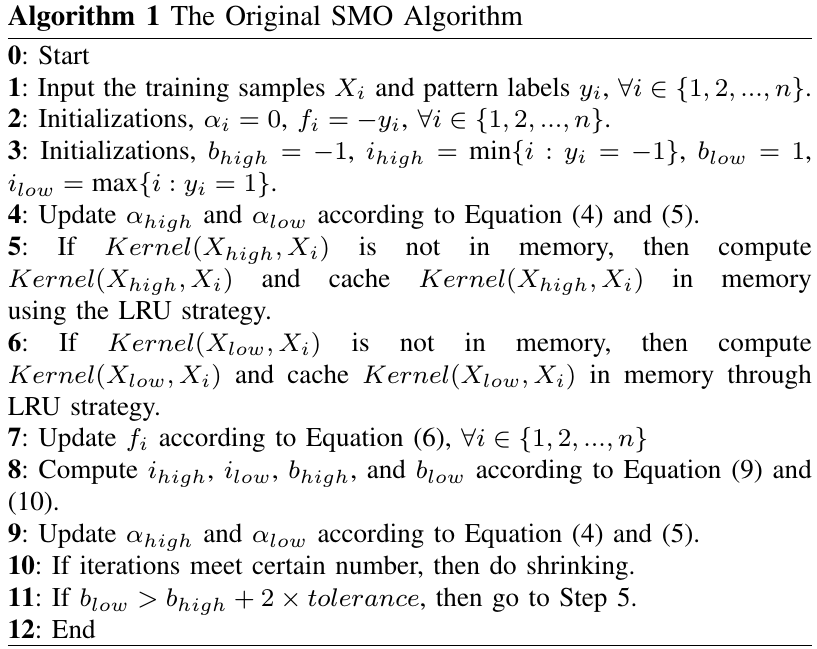
\includegraphics[width=0.8\textwidth]{figs/smo_algo.png}
		
		%\footnotesize {Logistic Regression}				
	\end{figure} 
\end{frame}

\begin{frame}
	\frametitle{SMO:Summary}	
	\begin{figure}
		%\includegraphics[width=0.6\textwidth]{fig/"l1l2".jpg}
		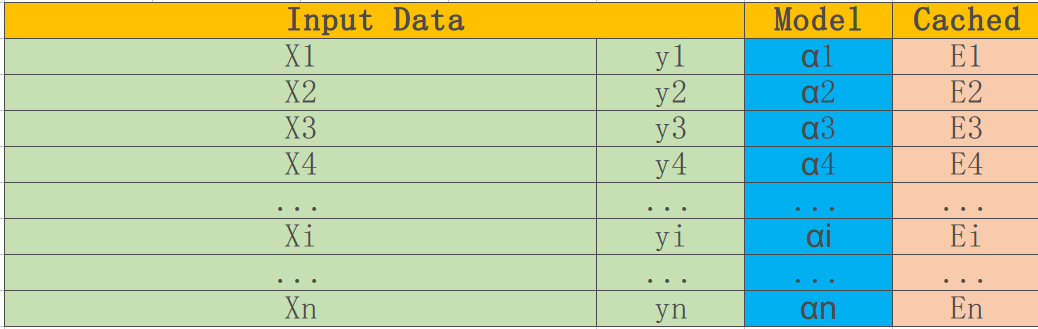
\includegraphics[width=0.9\textwidth]{figs/smo_datastructure.png}
		
		%\footnotesize {Logistic Regression}				
	\end{figure} 
	\begin{itemize}
		\item QP overall time complexity at least $O(n^{2})$, space $O(n^{2})$
		\item SMO type algorithm, empirically, it is known that the number of iterations may be higher than
		linear to the number of training data.
		\item $E_{i}^{new} = E_i + (\alpha_{1}^{new}-\alpha_1)y_1K(\vec{X_1},\vec{X_i}) + (\alpha_{2}^{new}-\alpha_2)y_2K(\vec{X_2},\vec{X_i})$
		\item The update of all $E_i$ at each
		step requires access to all the training samples, which costs more
		than 90\% of the total time in the entire SMO algorithm. 
		
		
	\end{itemize}
\end{frame}

\subsection{III. Methodology for MIC-SVM}

\begin{frame}
	\frametitle{Methodology to parallelizing and optimizing}
	\begin{itemize}
	\item In this section, we will briefly describe several important \textcolor{red}{design
	methods} and \textcolor{red}{optimization} details for our proposed MIC-SVM on
	parallelizing and accelerating SVM method on \textcolor{blue}{Intel Ivy Bridge CPUs}
	and \textcolor{purple}{Intel Xeon Phi coprocessor (MIC)}. 
		\begin{figure}
			%\includegraphics[width=0.6\textwidth]{fig/"l1l2".jpg}
			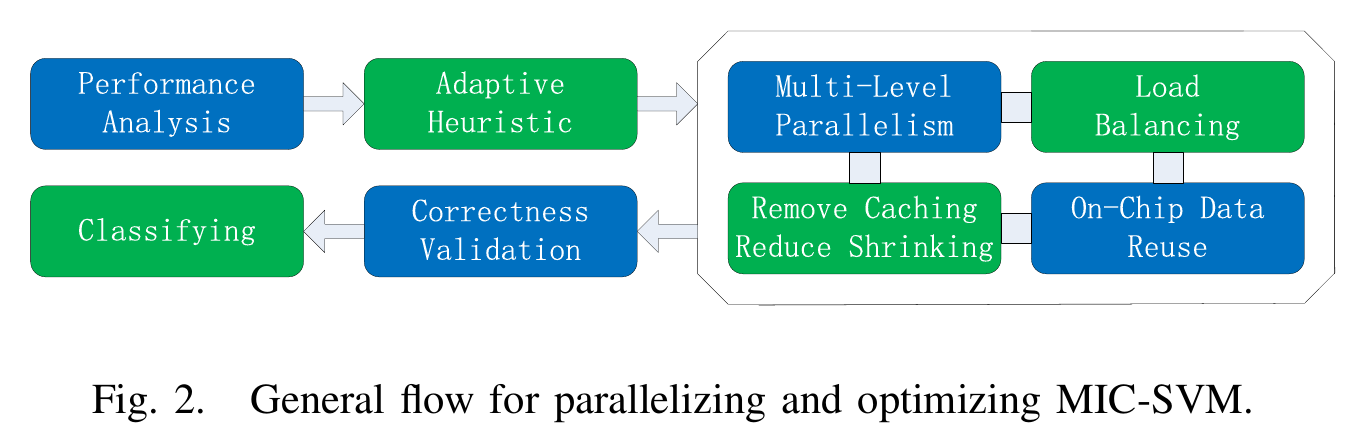
\includegraphics[width=0.9\textwidth]{figs/fig2_methodology.png}
			%\footnotesize {Logistic Regression}				
		\end{figure} 
	\end{itemize}	
\end{frame}


\begin{frame}
	\frametitle{A: Analysis of the Algorithm and Architecture}

	\begin{figure}
		%\includegraphics[width=0.6\textwidth]{fig/"l1l2".jpg}
		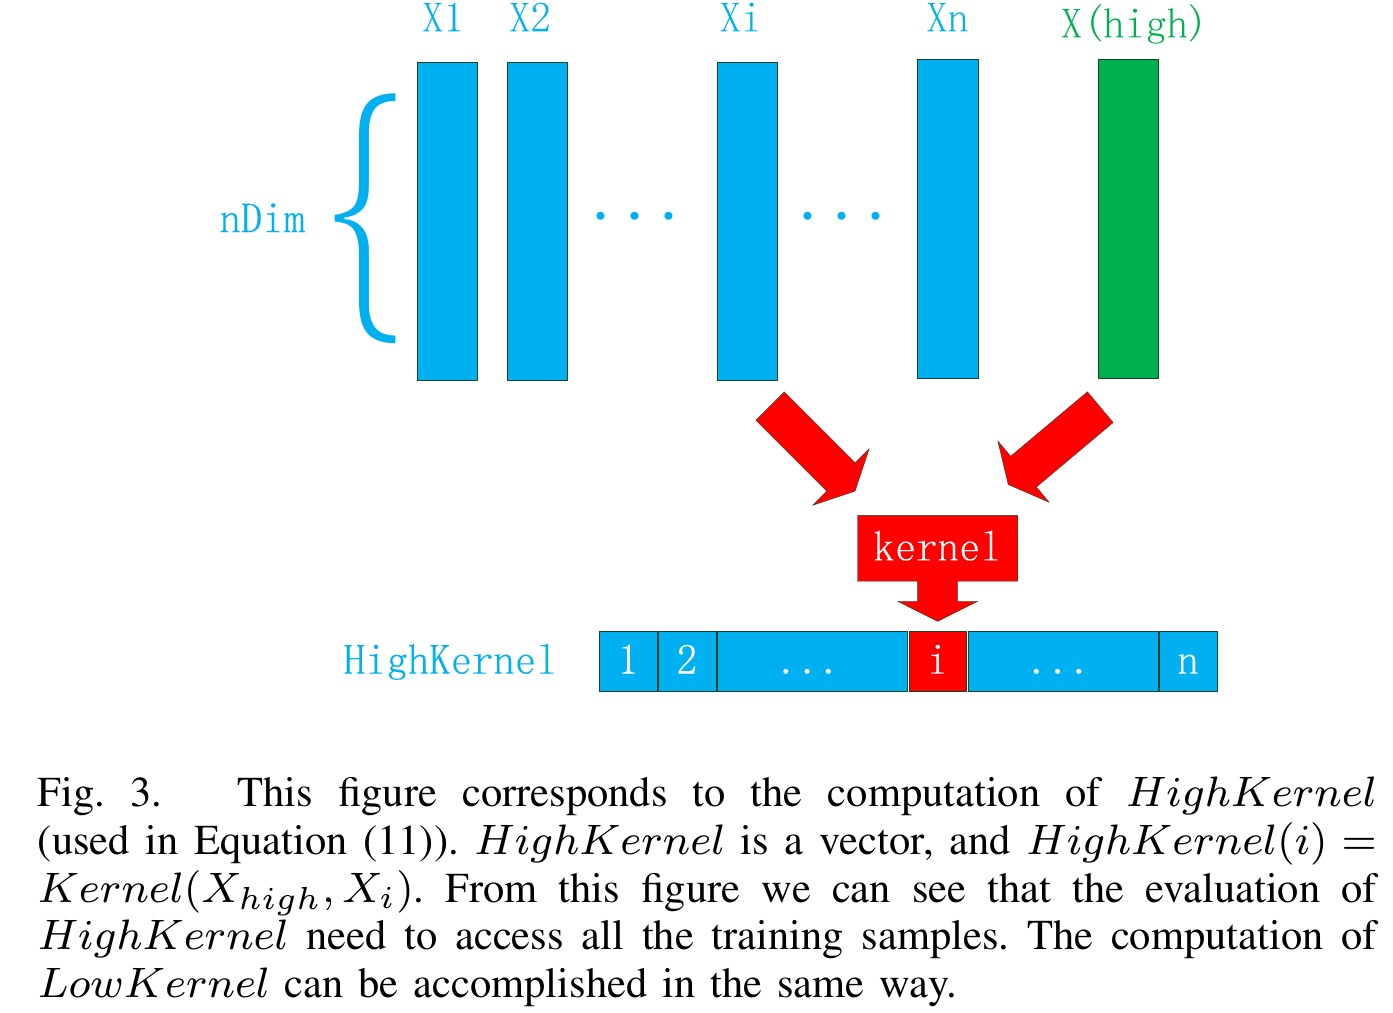
\includegraphics[width=0.6\textwidth]{figs/Fig3_CalcF.png}
		%\footnotesize {Logistic Regression}				
	\end{figure} 
	\begin{itemize}
		\item $E_{i}^{new} = E_i + (\alpha_{1}^{new}-\alpha_1)y_1K(\vec{X_1},\vec{X_i}) + (\alpha_{2}^{new}-\alpha_2)y_2K(\vec{X_2},\vec{X_i})$
		\item The update of all $E_i$ is the bottleneck. 
		\item \textcolor{red}{what's the bound?}
	\end{itemize}	
\end{frame}

\begin{frame}
	\frametitle{A: Analysis of the Algorithm and Architecture}
	\begin{columns}[c] % The "c" option specifies centered vertical alignment while the "t" option is used for top vertical alignment
		
		\column{.5\textwidth} % Left column and width
		%\textbf{Heading}
		\begin{figure}
			%\includegraphics[width=0.6\textwidth]{fig/"l1l2".jpg}
		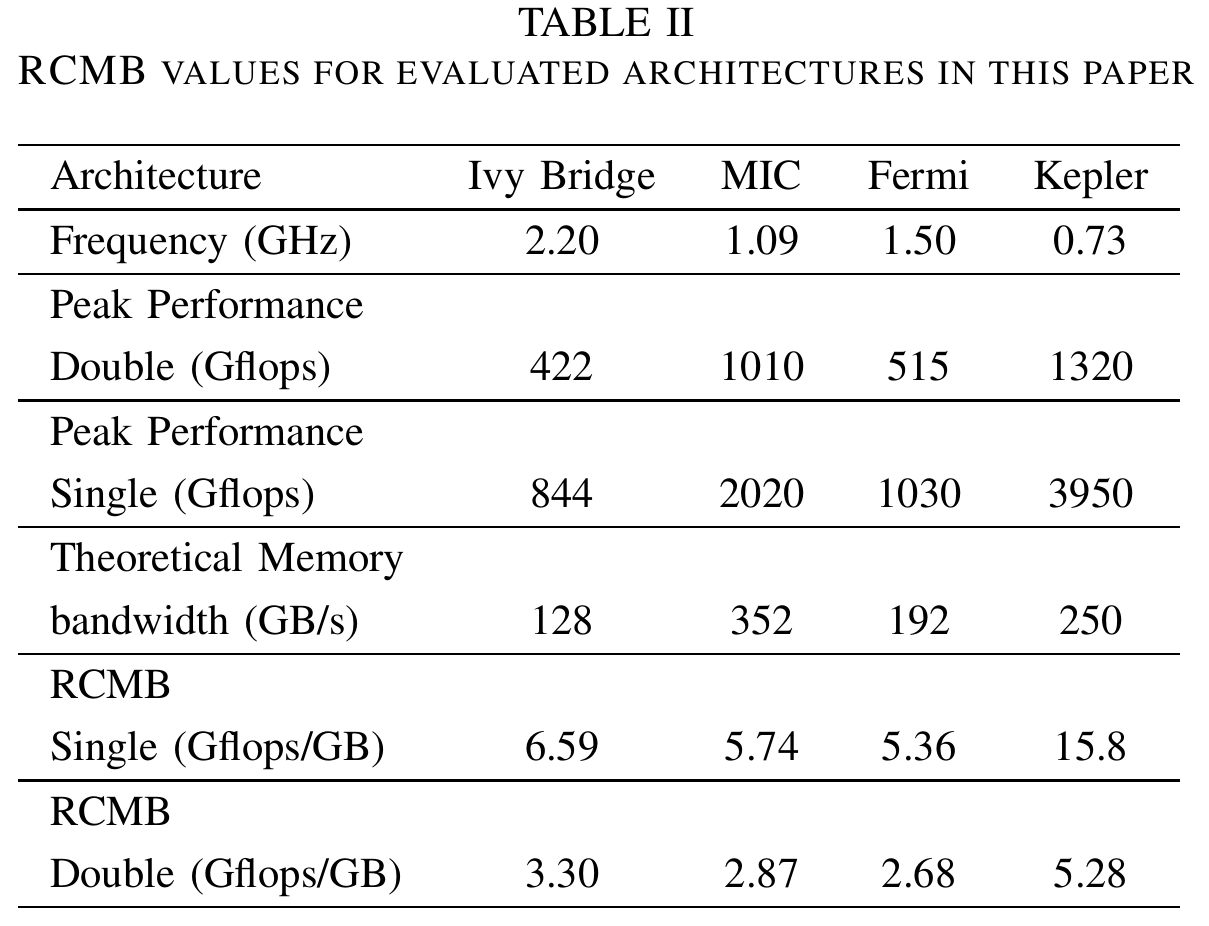
\includegraphics[width=0.8\textwidth]{figs/table2_rcmb.png}
			
			%\footnotesize {Logistic Regression}				
		\end{figure}
		
		\column{.5\textwidth} % Right column and width
			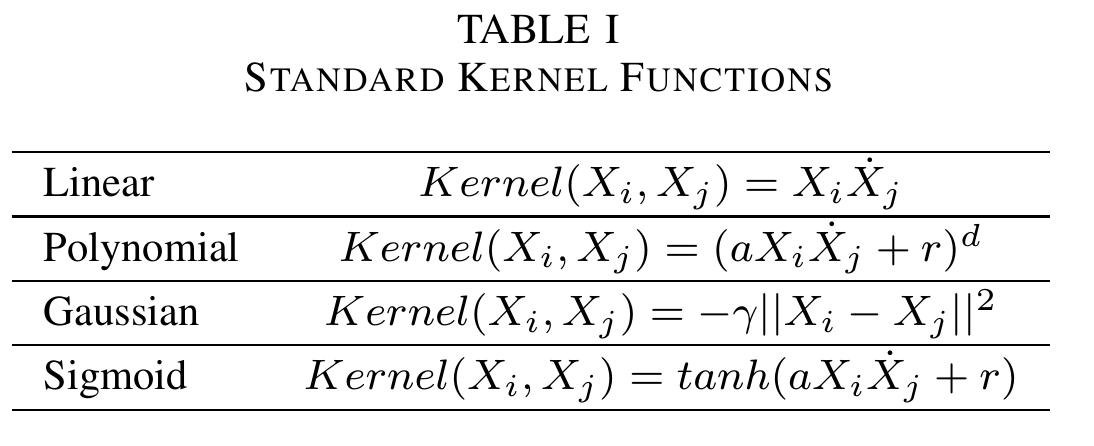
\includegraphics[width=0.8\textwidth]{figs/table1_kernel.png}
				

	\end{columns}	
	\begin{itemize}
		\item Define the \textcolor{red}{Ratio of Computation to Memory Access}
		(RCMA) to describe SMO’s algorithmic feature. \\
		$RCMA=\frac{number\_of\_comp\_flops}{number\_of\_memory\_access\_bytes}$
		\item Define Ratio of Peak Computation to Peak Memory Bandwidth (RCMB)
		to describe the theoretical architectural bound. \\ 
		$RCMB=\frac{theoretical\_peak\_performance}{theoretical\_bandwidth}$		
	\end{itemize}	
\end{frame}

\begin{frame}
	\frametitle{C: Two-Level Parallelism}
	\begin{table}[bt]
		\begin{tabular}{|p{2.4cm}|p{4cm}|p{4.4cm}|} \hline
		\textbf{arch} & \textbf{task parallelism}	& \textbf{data parallelism} \\ \hline	
		Ivy Bridge & utilizing multiple hardware threads & SIMD(AVX256) \\ \hline			
		MIC & utilizing multiple hardware threads & on-core VPU (Vector Processing Unit) and SIMD(AVX512) \\ \hline	
		%warps, groups of threads sharing instruction stream
		%Streaming Multiprocessor (SM):composed by 32 CUDA cores in fermi
		Fermi,Kepler & independent warps & different CUDA cores \\ \hline	
		\end{tabular}
	\end{table}					

\end{frame}

\begin{frame}
	\frametitle{C: Two-Level Parallelism}
	\begin{columns}[c] % The "c" option specifies centered vertical alignment while the "t" option is used for top vertical alignment
		\column{.5\textwidth} % Left column and width
		%\textbf{Heading}
		\begin{figure}
			%\includegraphics[width=0.6\textwidth]{fig/"l1l2".jpg}
			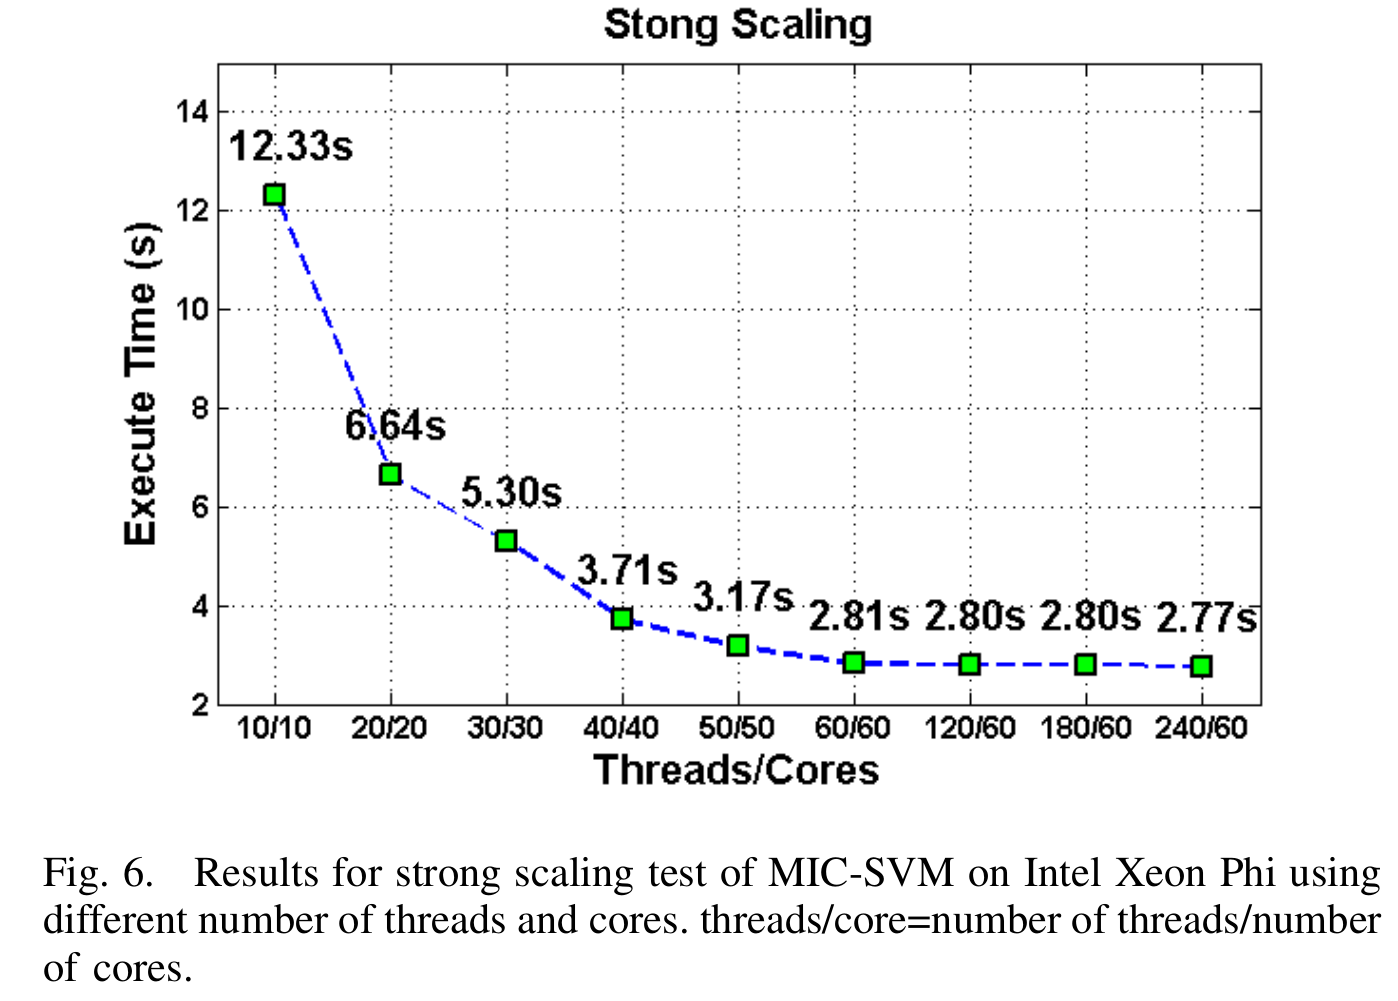
\includegraphics[width=0.9\textwidth]{figs/fig6_strongscaling.png} \\
			%\footnotesize {Logistic Regression}
			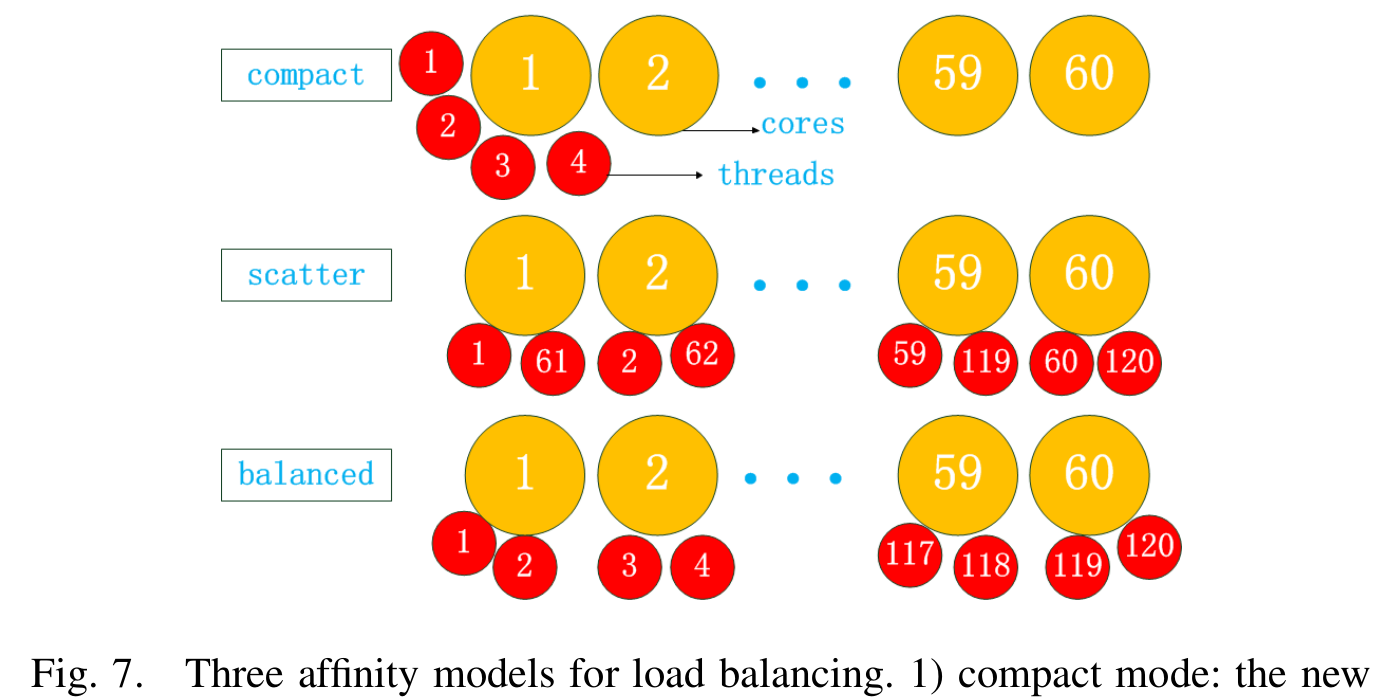
\includegraphics[width=0.9\textwidth]{figs/fig7_affinitymodel.png}
		\end{figure}
		\column{.5\textwidth} % Right column and width
		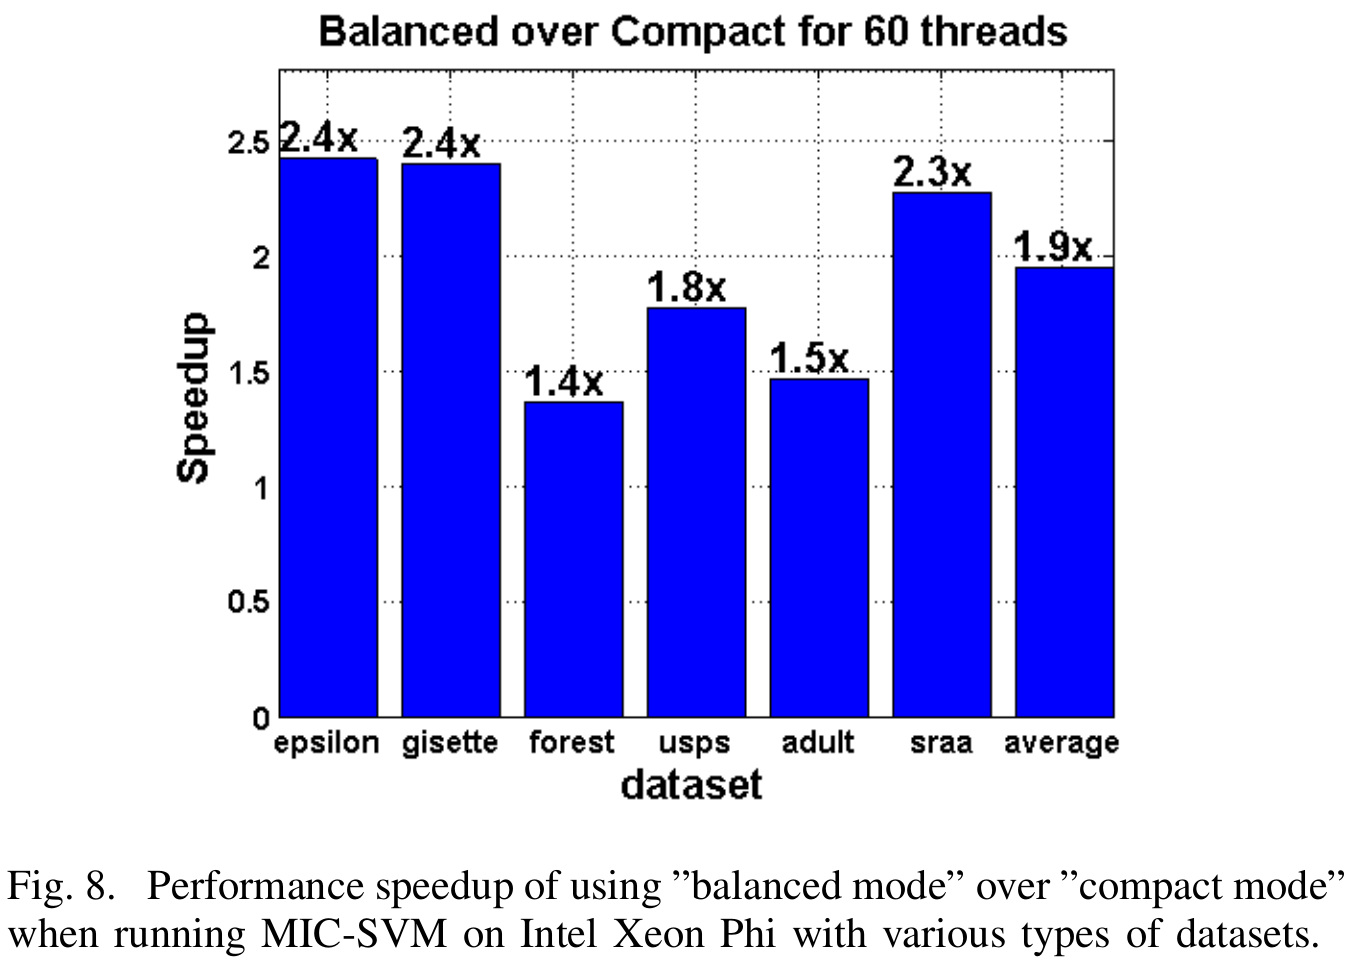
\includegraphics[width=0.9\textwidth]{figs/fig8_balancedmode.png}
		\begin{itemize}
			\item The proper number of threads: number of physical resources in device
			\item Load balancing: affinity models
			\item use the Cilk
			array notation to achieve the data parallelism explicitly rather than
			applying the implicit compiler model.
					
		\end{itemize}	
	\end{columns}	
\end{frame}

\begin{frame}
	\frametitle{D: Removing Caching and Reduce Shrinking Frequency}
	\begin{columns}[c] % The "c" option specifies centered vertical alignment while the "t" option is used for top vertical alignment
		\column{.5\textwidth} % Left column and width
		%\textbf{Heading}
		\begin{figure}
			%\includegraphics[width=0.6\textwidth]{fig/"l1l2".jpg}
			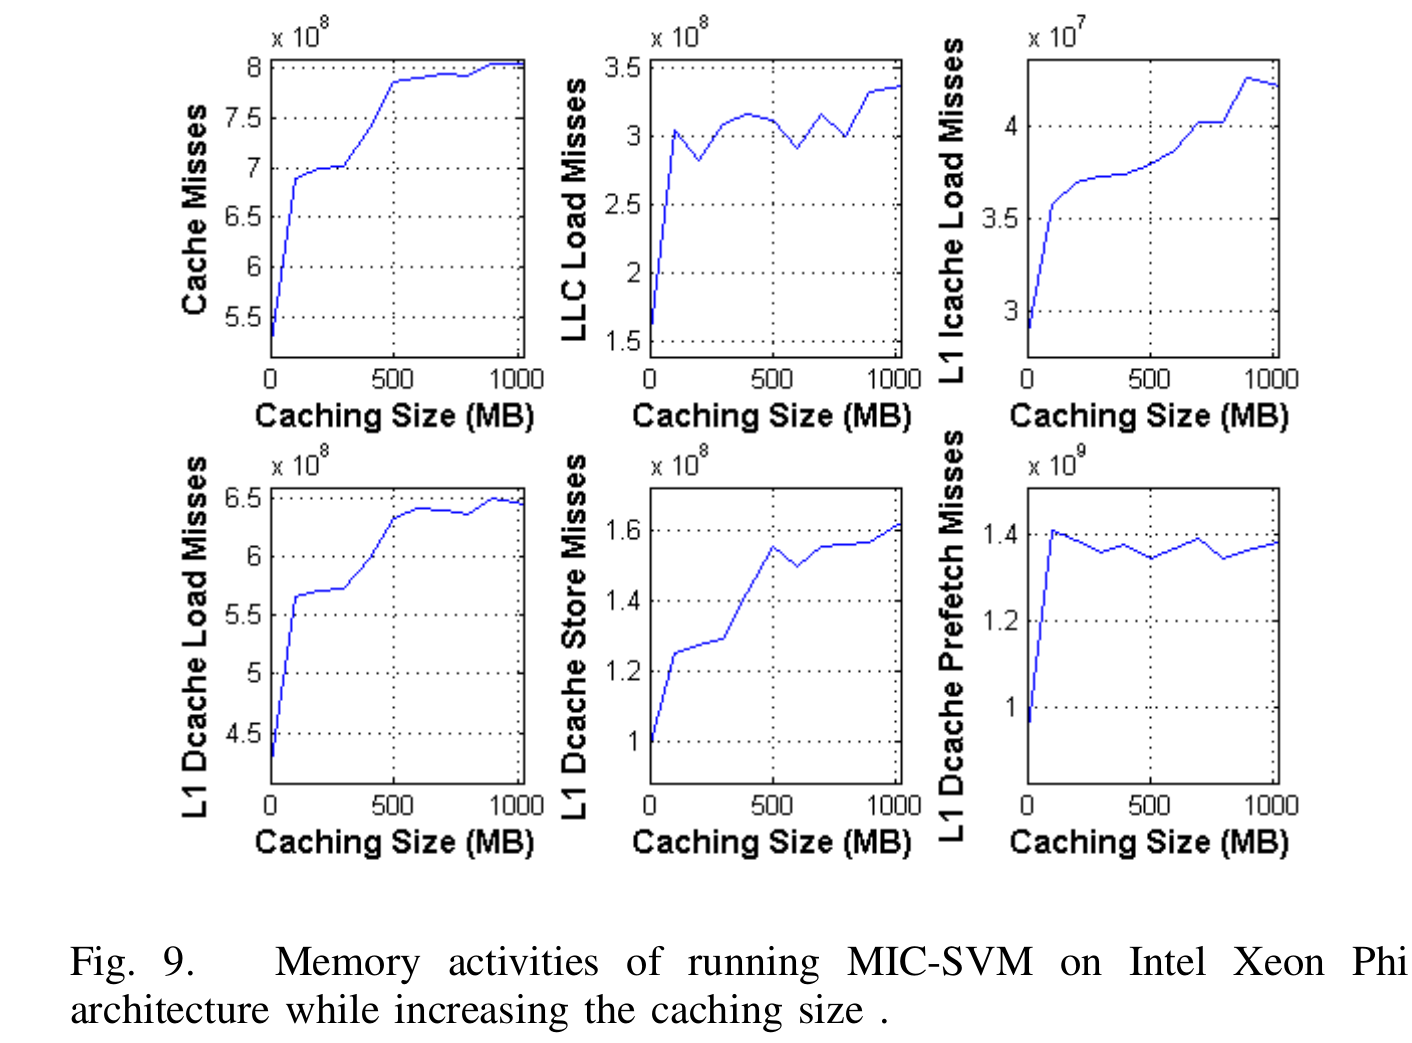
\includegraphics[width=1\textwidth]{figs/fig9_memorytraits.png}
		\end{figure}
		\column{.5\textwidth} % Right column and width
		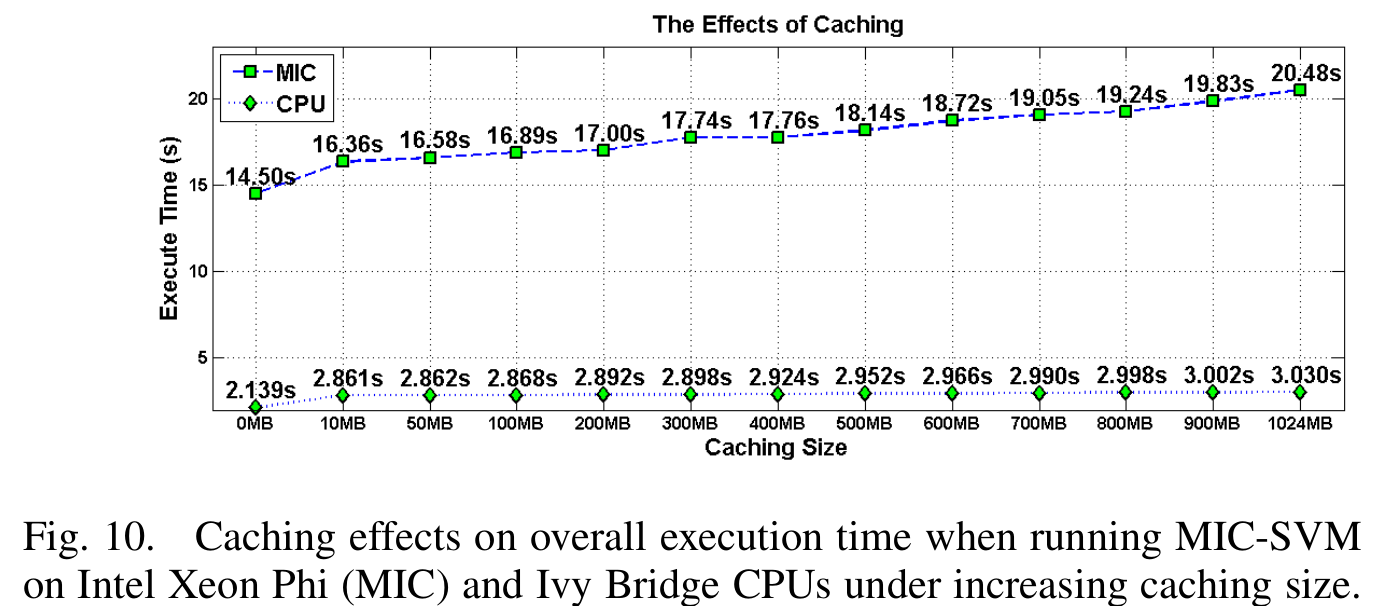
\includegraphics[width=1\textwidth]{figs/fig10_cache.png}

	\end{columns}	
		\begin{itemize}
			\item caching strategy can
			effectively reduce the number of kernels being evaluated. However,
			it also requires more memory access, may affect the performance negatively due to high memory
			access latency, memory contention from multithreading, and limited
			bandwidth. 			
		\end{itemize}		
\end{frame}

\begin{frame}
	\frametitle{E. Reducing the Gap Between RCMA and RCMB}
	\begin{itemize}
		%Static Schedules. By default, OpenMP statically assigns loop iterations to threads. When the parallel for block is entered, it assigns each thread the set of loop iterations it is to execute. This program also specifies static scheduling, in the parallel for directive.
		\item Together with load balancing, we employ the
		OpenMP SCHEDULE technique (static type, default chunk size)
		to \textcolor{red}{distribute the training samples evenly} to all hardware threads. 
		\item exploring the proper \textcolor{red}{granularity of
		parallelism} by configuring the data sizes for two-level parallelism,
		\item minimizing the threads’ creation and destroy to reduce synchronization overhead
		\item maximizing the \textcolor{red}{TLB page size} to 2MB to obtain
		significantly more memory coverage when the datasets require more
		than 16MB memory.	
		 			
	\end{itemize}		
\end{frame}

\begin{frame}
	\frametitle{Parallel SMO Algorithm}	
	\begin{figure}
		%\includegraphics[width=0.6\textwidth]{fig/"l1l2".jpg}
		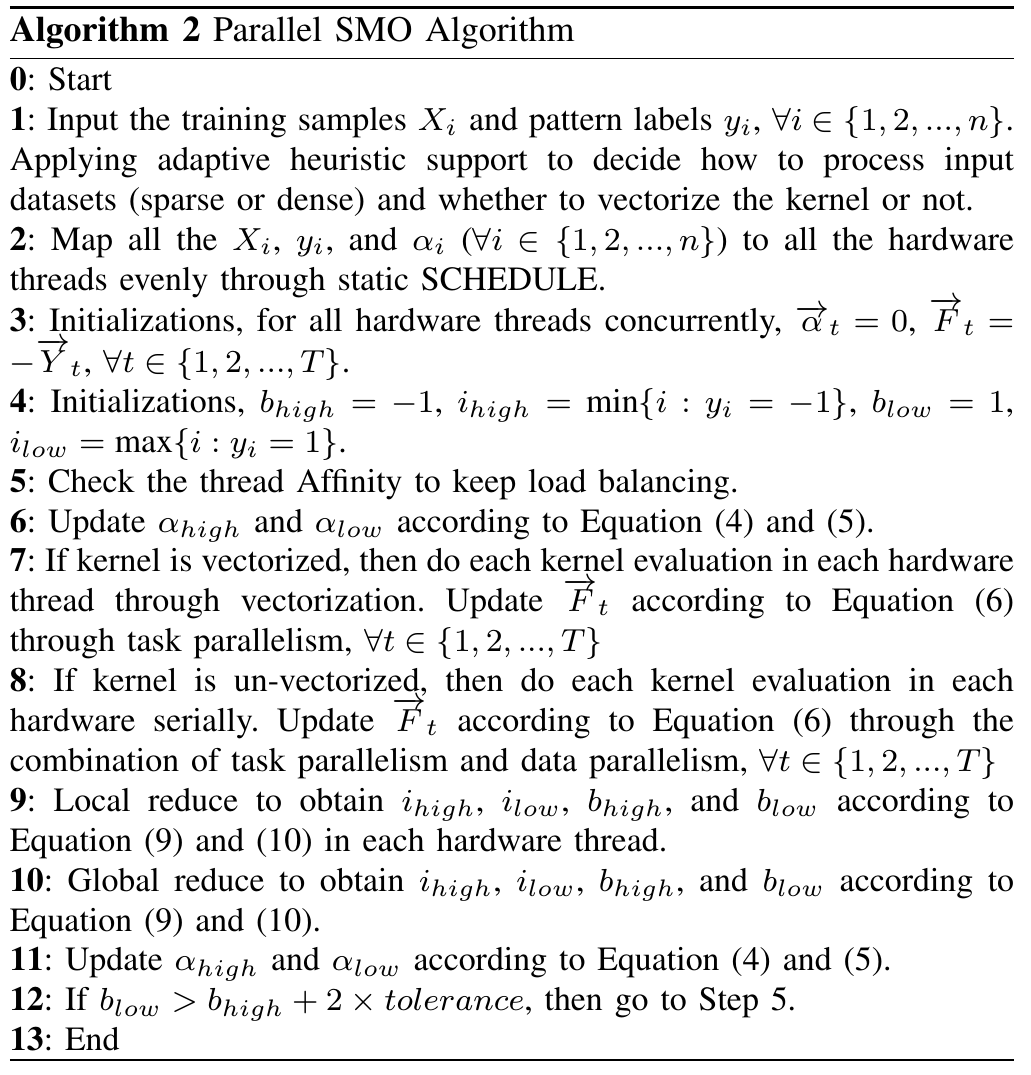
\includegraphics[width=0.6\textwidth]{figs/smo_parallelalgo.png}
		%\footnotesize {Logistic Regression}				
	\end{figure} 
\end{frame}

\subsection{IV. Experimental results and analysis} 
\begin{frame}
	\frametitle{A. Experimental Setup and Datasets}	
	\begin{figure}
		%\includegraphics[width=0.6\textwidth]{fig/"l1l2".jpg}
		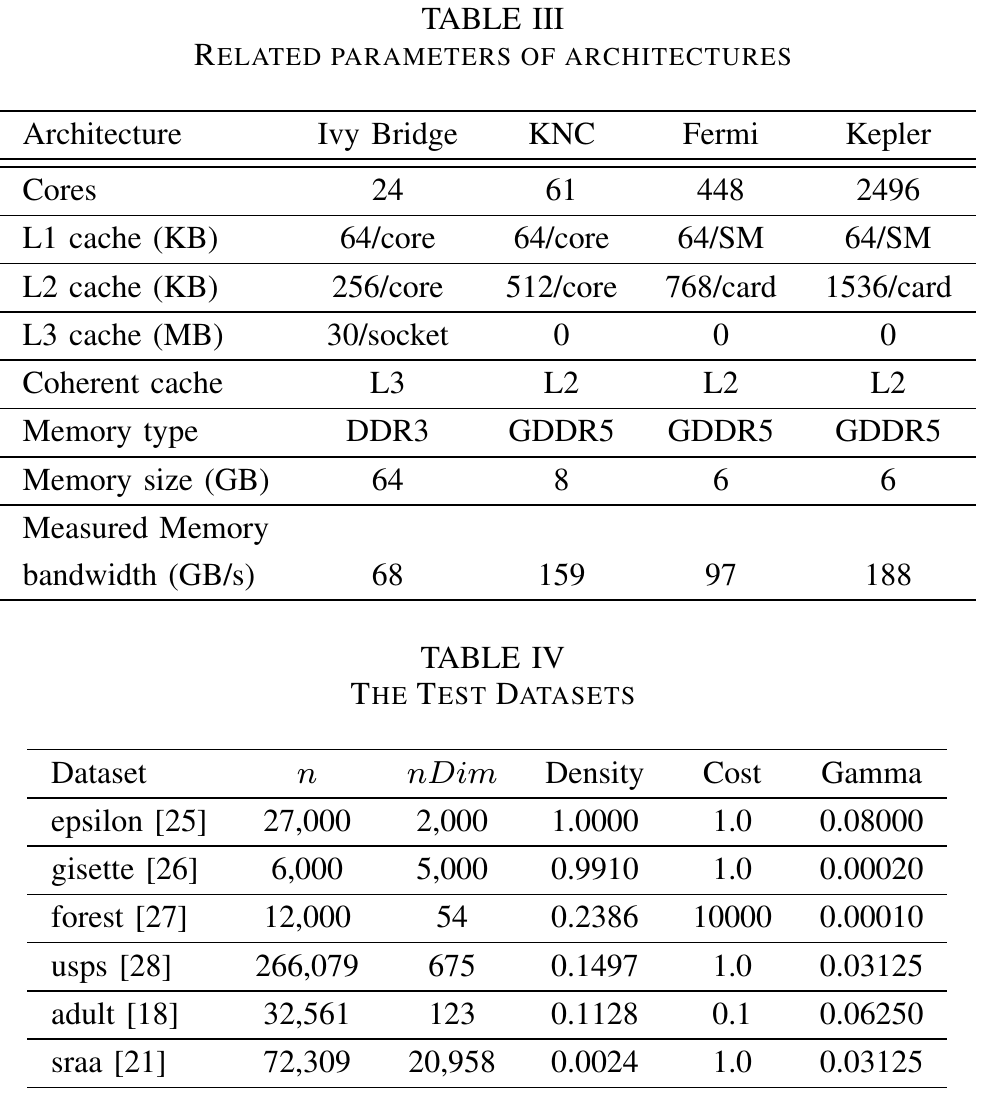
\includegraphics[width=0.6\textwidth]{figs/expsetup.png}
		%\footnotesize {Logistic Regression}				
	\end{figure} 
\end{frame}

\begin{frame}
	\frametitle{C. Correctness Validation for MIC-SVM}	
	\begin{figure}
		%\includegraphics[width=0.6\textwidth]{fig/"l1l2".jpg}
		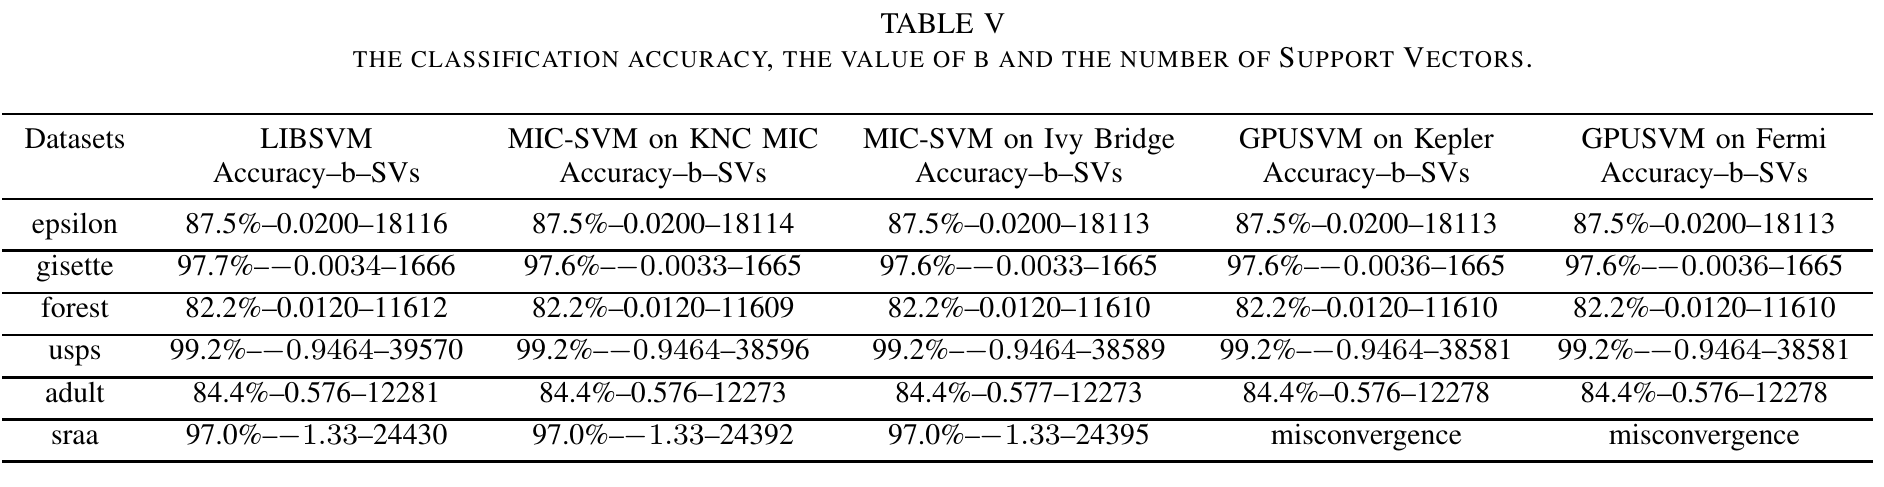
\includegraphics[width=1\textwidth]{figs/table5_accuracy}
		%\footnotesize {Logistic Regression}				
	\end{figure} 
	\begin{itemize}
		%Static Schedules. By default, OpenMP statically assigns loop iterations to threads. When the parallel for block is entered, it assigns each thread the set of loop iterations it is to execute. This program also specifies static scheduling, in the parallel for directive.
		\item baseline: serial LIBSVM
		\item another solver on gpu: GPUSVM	
		\item metrics: accuracy, support vectors number, b(discrepancy E)
		\item result: \textcolor{red}{nearly the same}
	\end{itemize}		
\end{frame}

\begin{frame}
	\frametitle{D. Performance Comparisons and Analysis}	
	\begin{figure}
		%\includegraphics[width=0.6\textwidth]{fig/"l1l2".jpg}
		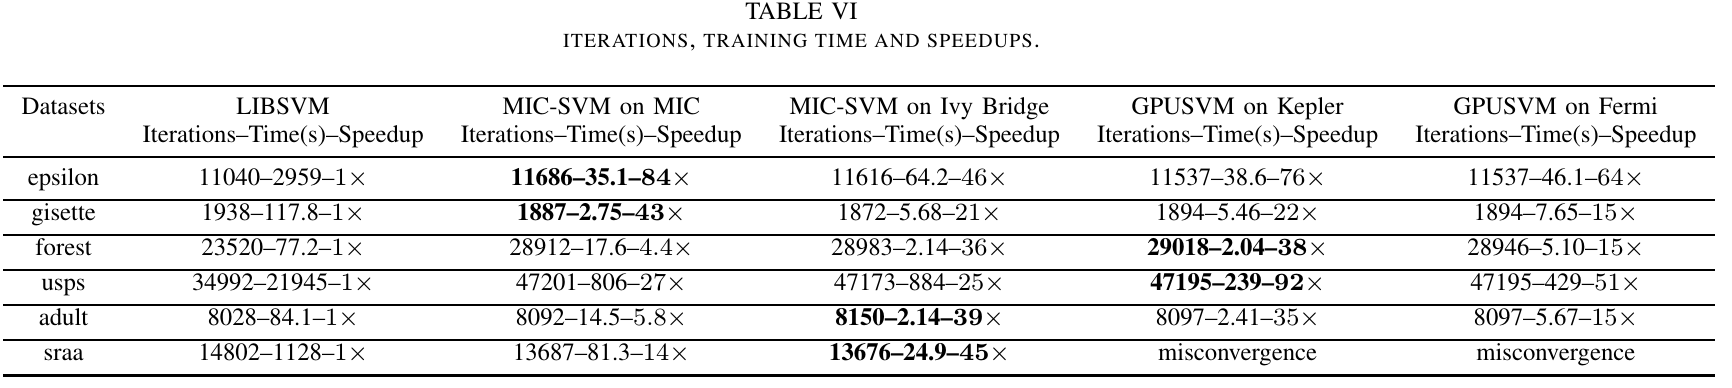
\includegraphics[width=1\textwidth]{figs/table6_performance}
		%\footnotesize {Logistic Regression}				
	\end{figure} 
	\begin{itemize}
		%Static Schedules. By default, OpenMP statically assigns loop iterations to threads. When the parallel for block is entered, it assigns each thread the set of loop iterations it is to execute. This program also specifies static scheduling, in the parallel for directive.
		\item With powerful SIMD mechanism (512 bits), MIC is
		a good candidate for the \textcolor{red}{dense high-dimension datasets} with \textcolor{blue}{modest
		number of training samples} because data parallelism can be achieved
		efficiently through vectorization; 
		\item Equipped with sufficient caches and high clock frequency, Ivy Bridge CPUs are suitable for \textcolor{red}{sparse
		high-dimension datasets} since these datasets often require coarse-grained parallel processing; 
		\item GPUs are proper for the datasets with
		\textcolor{blue}{large number of training samples} and \textcolor{red}{low dimension} because they
		are more likely to benefit from millions of fine-grained lightweight
		threads.
		
		
		
	\end{itemize}		
\end{frame}

\begin{frame}
	\frametitle{D. Performance Comparisons and Analysis}	
	\begin{figure}
		%\includegraphics[width=0.6\textwidth]{fig/"l1l2".jpg}
		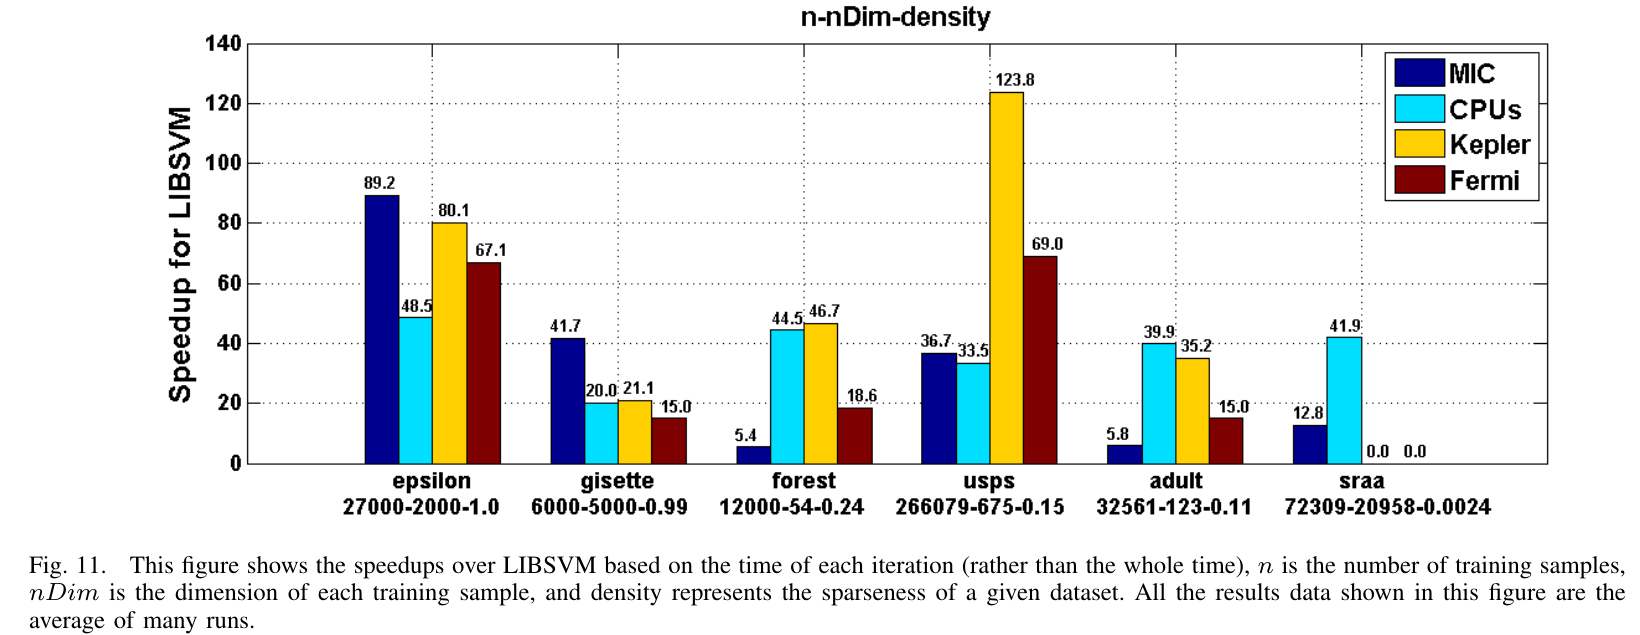
\includegraphics[width=1\textwidth]{figs/fig11_speedup}
		%\footnotesize {Logistic Regression}				
	\end{figure} 

\end{frame}

\subsection{VI. Conclusion} 
\begin{frame}
	\frametitle{Conclusion}	
	\begin{block}{Conclusion}
		\begin{itemize}
			\item propose MIC-SVM, a highly efficient parallel
			support vector machine for x86 based multi-core and many-core
			architectures such as Intel Ivy Bridge CPUs and Intel KNC MIC.
			\item propose various novel analysis and optimization strategies that
			are general and can be easily applied to accelerate other machine
			learning methods. 
			\item explore and improve the deficiencies of
			the current SVM tools. 
			\item provide insights on how to map the
			most suitable architectures to specific data patterns in order to achieve the best performance. 
		\end{itemize}		
	\end{block}
	\begin{block}{Future work}
		\begin{itemize}
			\item In future, we plan to extend the current MIC-SVM to distributed memory environment using multiple MICs. 
		
		\end{itemize}		
	\end{block}
	
\end{frame}

\section{Comments} % Sections 
\subsection{Pros and Cons} 

\begin{frame}
	\frametitle{Comments on the paper}
	\begin{block}{Pros}
		\begin{itemize}
			\item gives a clear structure of the process of investigation.
			\item experiments are concise and informative. 
			\item gives general analysis method and insights, which will be helpful to the community. 
		\end{itemize}		
	\end{block}
	\begin{block}{Cons}
		\begin{itemize}
			\item well known optimizing techniques, and plain results, no much exciting things
			\item limited details on the effectiveness of optimizing techniques, e.g., the solution to fill the gap of RCMA and RCMB should be very cool, but...			
		\end{itemize}		
	\end{block}
\end{frame}
%------------------------------------------------
%appendix

%------------------------------------------------

\begin{frame}
\frametitle{References}
%This statement requires citation \cite{p1}.
\footnotesize{
\begin{thebibliography}{99} % Beamer does not support BibTeX so references must be inserted manually as below
%\bibitem[Smith, 2012]{p1} John Smith (2012)
%\newblock Title of the publication
%\newblock \emph{Journal Name} 12(3), 45 -- 678.

\bibitem[Platt 1998]{Platt} Platt, J., 1998. Sequential minimal optimization: A fast algorithm for training support vector machines.

\bibitem[You 2014]{You} Y. You et al., “Mic-svm: Designing a highly efficient support vector machine for advanced modern multi-core and many-core architectures,” in Parallel and Distributed Processing Symposium, 2014 IEEE 28th International, 2014, pp. 809–818.

\end{thebibliography}
}
\end{frame}



%------------------------------------------------

\begin{frame}
\Huge{\centerline{The End}}
\end{frame}

%----------------------------------------------------------------------------------------

\end{document} 
